\section{逼真相机}\label{sec:逼真相机}
\begin{remark}
    本节含有高级内容,第一次阅读时可以跳过。
\end{remark}

薄透镜模型使得能渲染因景深而模糊的图像,
但它只是对多个\keyindex{透镜元件}{lens element}{}构成的
真实相机透镜系统非常粗糙的近似,而每个透镜元件都会改变穿过它的辐射分布
(\reffig{6.15}展示了具有8个元件的22mm焦距\keyindex{广角}{wide-angle}{}镜头横截面)。
即使基本的手机相机也趋于有五个左右独立的透镜元件,
而\keyindex{数码单镜头反光相机}{digital single-lens reflex camera}{camera相机}
(数码单反相机,DSLR)镜头可能有十个或更多。
通常,具备更大数量透镜元件的更复杂透镜系统能
比更简单的透镜系统创建更高质量的图像。
\begin{figure}[htbp]
    \centering%LaTeX with PSTricks extensions
%%Creator: Inkscape 1.1.1 (3bf5ae0d25, 2021-09-20)
%%Please note this file requires PSTricks extensions
\psset{xunit=.5pt,yunit=.5pt,runit=.5pt}
\begin{pspicture}(480,210.66666667)
{
\newrgbcolor{curcolor}{0 0 0}
\pscustom[linewidth=1.33333333,linecolor=curcolor]
{
\newpath
\moveto(102.07812533,200.869792)
\curveto(80.78645867,139.869792)(80.78645867,73.46354133)(102.07812533,12.46354133)
}
}
{
\newrgbcolor{curcolor}{0 0 0}
\pscustom[linewidth=1.33333333,linecolor=curcolor]
{
\newpath
\moveto(102.125,200.34895867)
\lineto(129.375,200.34895867)
}
}
{
\newrgbcolor{curcolor}{0 0 0}
\pscustom[linewidth=1.33333333,linecolor=curcolor]
{
\newpath
\moveto(102.125,11.942708)
\lineto(129.375,11.942708)
}
}
{
\newrgbcolor{curcolor}{0 0 0}
\pscustom[linewidth=1.33333333,linecolor=curcolor]
{
\newpath
\moveto(129.375,200.34895867)
\lineto(129.375,177.625)
}
}
{
\newrgbcolor{curcolor}{0 0 0}
\pscustom[linewidth=1.33333333,linecolor=curcolor]
{
\newpath
\moveto(129.375,11.942708)
\lineto(129.375,34.66145867)
}
}
{
\newrgbcolor{curcolor}{0 0 0}
\pscustom[linewidth=1.33333333,linecolor=curcolor]
{
\newpath
\moveto(129.95833333,178.14583333)
\curveto(108.70312533,160.494792)(96.41145867,134.29687467)(96.41145867,106.66666667)
\curveto(96.41145867,79.03645867)(108.70312533,52.83854133)(129.95833333,35.1875)
}
}
{
\newrgbcolor{curcolor}{0 0 0}
\pscustom[linewidth=1.33333333,linecolor=curcolor]
{
\newpath
\moveto(187.03125067,155.77604133)
\curveto(170.58854133,125.09895867)(170.58854133,88.23437467)(187.03125067,57.557292)
}
}
{
\newrgbcolor{curcolor}{0 0 0}
\pscustom[linewidth=1.33333333,linecolor=curcolor]
{
\newpath
\moveto(187.5625,155.255208)
\lineto(211.682292,155.255208)
}
}
{
\newrgbcolor{curcolor}{0 0 0}
\pscustom[linewidth=1.33333333,linecolor=curcolor]
{
\newpath
\moveto(187.5625,57.03125067)
\lineto(211.682292,57.03125067)
}
}
{
\newrgbcolor{curcolor}{0 0 0}
\pscustom[linewidth=1.33333333,linecolor=curcolor]
{
\newpath
\moveto(211.682292,155.255208)
\lineto(211.682292,145.119792)
}
}
{
\newrgbcolor{curcolor}{0 0 0}
\pscustom[linewidth=1.33333333,linecolor=curcolor]
{
\newpath
\moveto(211.682292,57.03125067)
\lineto(211.682292,67.17187467)
}
}
{
\newrgbcolor{curcolor}{0 0 0}
\pscustom[linewidth=1.33333333,linecolor=curcolor]
{
\newpath
\moveto(211.52604133,67.692708)
\curveto(217.22916667,93.364584)(217.22916667,119.96874933)(211.52604133,145.64062533)
}
}
{
\newrgbcolor{curcolor}{0 0 0}
\pscustom[linewidth=1.33333333,linecolor=curcolor]
{
\newpath
\moveto(211.682292,145.119792)
\lineto(231.1875,145.119792)
}
}
{
\newrgbcolor{curcolor}{0 0 0}
\pscustom[linewidth=1.33333333,linecolor=curcolor]
{
\newpath
\moveto(211.682292,67.17187467)
\lineto(231.1875,67.17187467)
}
}
{
\newrgbcolor{curcolor}{0 0 0}
\pscustom[linewidth=1.33333333,linecolor=curcolor]
{
\newpath
\moveto(231.1875,145.119792)
\lineto(231.1875,142.5)
}
}
{
\newrgbcolor{curcolor}{0 0 0}
\pscustom[linewidth=1.33333333,linecolor=curcolor]
{
\newpath
\moveto(231.1875,67.17187467)
\lineto(231.1875,69.79166667)
}
}
{
\newrgbcolor{curcolor}{0 0 0}
\pscustom[linewidth=1.33333333,linecolor=curcolor]
{
\newpath
\moveto(231.33333333,143.02083333)
\curveto(229.77083333,118.807292)(229.77083333,94.52604133)(231.33333333,70.3125)
}
}
{
\newrgbcolor{curcolor}{0 0 0}
\pscustom[linewidth=2.66666667,linecolor=curcolor]
{
\newpath
\moveto(236.510416,140.92708267)
\lineto(236.510416,175.70312533)
}
}
{
\newrgbcolor{curcolor}{0 0 0}
\pscustom[linewidth=2.66666667,linecolor=curcolor]
{
\newpath
\moveto(236.510416,71.364584)
\lineto(236.510416,36.58333333)
}
}
{
\newrgbcolor{curcolor}{0 0 0}
\pscustom[linewidth=1.33333333,linecolor=curcolor]
{
\newpath
\moveto(247.53125067,74.15625067)
\curveto(257.25,94.739584)(257.25,118.59374933)(247.53125067,139.17708267)
}
}
{
\newrgbcolor{curcolor}{0 0 0}
\pscustom[linewidth=1.33333333,linecolor=curcolor]
{
\newpath
\moveto(247.32291733,142.5)
\lineto(266.23437467,142.5)
}
}
{
\newrgbcolor{curcolor}{0 0 0}
\pscustom[linewidth=1.33333333,linecolor=curcolor]
{
\newpath
\moveto(247.32291733,69.79166667)
\lineto(266.23437467,69.79166667)
}
}
{
\newrgbcolor{curcolor}{0 0 0}
\pscustom[linewidth=1.33333333,linecolor=curcolor]
{
\newpath
\moveto(247.32291733,142.5)
\lineto(247.32291733,138.65104133)
}
}
{
\newrgbcolor{curcolor}{0 0 0}
\pscustom[linewidth=1.33333333,linecolor=curcolor]
{
\newpath
\moveto(247.32291733,69.79166667)
\lineto(247.32291733,73.635416)
}
}
{
\newrgbcolor{curcolor}{0 0 0}
\pscustom[linewidth=1.33333333,linecolor=curcolor]
{
\newpath
\moveto(265.98437467,70.3125)
\curveto(276.25,93.46354133)(276.25,119.869792)(265.98437467,143.02083333)
}
}
{
\newrgbcolor{curcolor}{0 0 0}
\pscustom[linewidth=1.33333333,linecolor=curcolor]
{
\newpath
\moveto(273.57812533,64.369792)
\curveto(274.47916667,92.5625)(274.47916667,120.77083333)(273.57812533,148.96354133)
}
}
{
\newrgbcolor{curcolor}{0 0 0}
\pscustom[linewidth=1.33333333,linecolor=curcolor]
{
\newpath
\moveto(274.17187467,151.58854133)
\lineto(278.78125067,151.58854133)
}
}
{
\newrgbcolor{curcolor}{0 0 0}
\pscustom[linewidth=1.33333333,linecolor=curcolor]
{
\newpath
\moveto(274.17187467,60.70312533)
\lineto(278.78125067,60.70312533)
}
}
{
\newrgbcolor{curcolor}{0 0 0}
\pscustom[linewidth=1.33333333,linecolor=curcolor]
{
\newpath
\moveto(274.17187467,151.58854133)
\lineto(274.17187467,148.442708)
}
}
{
\newrgbcolor{curcolor}{0 0 0}
\pscustom[linewidth=1.33333333,linecolor=curcolor]
{
\newpath
\moveto(274.17187467,60.70312533)
\lineto(274.17187467,63.84895867)
}
}
{
\newrgbcolor{curcolor}{0 0 0}
\pscustom[linewidth=1.33333333,linecolor=curcolor]
{
\newpath
\moveto(278.3125,61.22395867)
\curveto(291.4375,72.67708267)(298.97395867,89.244792)(298.97395867,106.66666667)
\curveto(298.97395867,124.08854133)(291.4375,140.65625067)(278.3125,152.10937467)
}
}
{
\newrgbcolor{curcolor}{0 0 0}
\pscustom[linewidth=1.33333333,linecolor=curcolor]
{
\newpath
\moveto(278.78125067,154.90625067)
\lineto(300.739584,154.90625067)
}
}
{
\newrgbcolor{curcolor}{0 0 0}
\pscustom[linewidth=1.33333333,linecolor=curcolor]
{
\newpath
\moveto(278.78125067,57.385416)
\lineto(300.739584,57.385416)
}
}
{
\newrgbcolor{curcolor}{0 0 0}
\pscustom[linewidth=1.33333333,linecolor=curcolor]
{
\newpath
\moveto(278.78125067,154.90625067)
\lineto(278.78125067,151.58854133)
}
}
{
\newrgbcolor{curcolor}{0 0 0}
\pscustom[linewidth=1.33333333,linecolor=curcolor]
{
\newpath
\moveto(278.78125067,57.385416)
\lineto(278.78125067,60.70312533)
}
}
{
\newrgbcolor{curcolor}{0 0 0}
\pscustom[linewidth=1.33333333,linecolor=curcolor]
{
\newpath
\moveto(301.28125067,57.90625067)
\curveto(313.60937467,89.244792)(313.60937467,124.08854133)(301.28125067,155.42708267)
}
}
{
\newrgbcolor{curcolor}{0 0 0}
\pscustom[linewidth=1.33333333,linecolor=curcolor]
{
\newpath
\moveto(310.05208267,53.35937467)
\curveto(329.29166667,64.20833333)(341.192708,84.57812533)(341.192708,106.66666667)
\curveto(341.192708,128.755208)(329.29166667,149.125)(310.05208267,159.97395867)
}
}
{
\newrgbcolor{curcolor}{0 0 0}
\pscustom[linewidth=1.33333333,linecolor=curcolor]
{
\newpath
\moveto(310.46354133,177.625)
\lineto(318.90104133,177.625)
}
}
{
\newrgbcolor{curcolor}{0 0 0}
\pscustom[linewidth=1.33333333,linecolor=curcolor]
{
\newpath
\moveto(310.46354133,34.66145867)
\lineto(318.90104133,34.66145867)
}
}
{
\newrgbcolor{curcolor}{0 0 0}
\pscustom[linewidth=1.33333333,linecolor=curcolor]
{
\newpath
\moveto(310.46354133,177.625)
\lineto(310.46354133,159.45312533)
}
}
{
\newrgbcolor{curcolor}{0 0 0}
\pscustom[linewidth=1.33333333,linecolor=curcolor]
{
\newpath
\moveto(310.46354133,34.66145867)
\lineto(310.46354133,52.83854133)
}
}
{
\newrgbcolor{curcolor}{0 0 0}
\pscustom[linewidth=1.33333333,linecolor=curcolor]
{
\newpath
\moveto(318.75,35.1875)
\curveto(339.32291733,53.244792)(351.114584,79.29166667)(351.114584,106.66666667)
\curveto(351.114584,134.04166667)(339.32291733,160.08854133)(318.75,178.14583333)
}
}
{
\newrgbcolor{curcolor}{0 0 0}
\pscustom[linewidth=1.33333333,linecolor=curcolor]
{
\newpath
\moveto(469.09374933,10.8125)
\lineto(469.09374933,201.47395867)
}
}
{
\newrgbcolor{curcolor}{0 0 0}
\pscustom[linewidth=1.33333333,linecolor=curcolor]
{
\newpath
\moveto(469.09374933,106.14583333)
\lineto(9.57291733,106.14583333)
}
}
\end{pspicture}

    \caption{广角透镜系统的横截面(在pbrt发行版的{\ttfamily scenes/lenses/wide.22mm.dat}
    中)。透镜坐标系统让胶片平面垂直于$z$轴且位于$z=0$处。
    透镜在左边负z轴上,然后场景在透镜左侧。透镜系统中部表示为粗黑线的光圈阻挡命中它的光线。
    在许多透镜系统中,可以调整光圈大小以在更短曝光时间(大光圈)和更大景深(小光圈)间权衡。}
    \label{fig:6.15}
\end{figure}

本节讨论\refvar{RealisticCamera}{}的实现,
它模拟光穿过像\reffig{6.15}那样的透镜系统后聚焦并渲染像\reffig{6.16}那样的图像。
其实现基于光线追踪,即相机追随光路穿过透镜元件,
并考虑具有不同折射率的介质(空气,各类玻璃)间界面的折射,
直到光路要么退出光学系统要么被光圈或镜头罩吸收。
离开前端镜头元件的光线代表相机响应曲线,可用于估计
沿任意光线入射辐亮度的积分器,例如\refvar{SamplerIntegrator}{}。
\refvar{RealisticCamera}{}的实现在文件\href{https://github.com/mmp/pbrt-v3/tree/master/src/cameras/realistic.h}{\ttfamily cameras/realistic.h}
和\href{https://github.com/mmp/pbrt-v3/tree/master/src/cameras/realistic.cpp}{\ttfamily cameras/realistic.cpp}中。
\begin{figure}[htbp]
    \centering\includegraphics[width=0.6\linewidth]{chap06/sanmiguel-fisheye.png}
    \caption{用鱼眼透镜和很宽视场渲染的图像。注意边缘暗处是
        准确模拟成像辐射度量(\refsub{相机测量方程})所致,
        而直线扭曲为曲线则是许多广角镜头的特点,但在用投影矩阵表示透镜投影模型时没有考虑。}
    \label{fig:6.16}
\end{figure}
\begin{lstlisting}
`\initcode{RealisticCamera Declarations}{=}`
class `\initvar{RealisticCamera}{}` : public `\refvar{Camera}{}` {
public:
    `\refcode{RealisticCamera Public Methods}{}`
private:
    `\refcode{RealisticCamera Private Declarations}{}`
    `\refcode{RealisticCamera Private Data}{}`
    `\refcode{RealisticCamera Private Methods}{}`
};
\end{lstlisting}

除了把相机放置于场景中的常见变换、\refvar{Film}{}以及快门打开和关闭的时间外,
\refvar{RealisticCamera}{}构造函数还接收透镜系统描述文件的文件名、
到期望的焦平面的距离以及光圈直径。之后有了第\refchap{蒙特卡洛积分}蒙特卡洛积分与
\refsub{相机测量方程}成像辐射度量的预备知识后,
将在\refsub{采样相机1}介绍参数{\ttfamily simpleWeighting}的作用。
\begin{lstlisting}
`\initcode{RealisticCamera Method Definitions}{=}\initnext{RealisticCameraMethodDefinitions}`
`\refvar{RealisticCamera}{}`::`\refvar{RealisticCamera}{}`(const `\refvar{AnimatedTransform}{}` &CameraToWorld,
        `\refvar{Float}{}` shutterOpen, `\refvar{Float}{}` shutterClose, `\refvar{Float}{}` apertureDiameter,
        `\refvar{Float}{}` focusDistance, bool simpleWeighting, const char *lensFile,
        `\refvar{Film}{}` *film, const `\refvar{Medium}{}` *medium)
    : `\refvar{Camera}{}`(CameraToWorld, shutterOpen, shutterClose, film, medium),
      simpleWeighting(simpleWeighting) {
    `\refcode{Load element data from lens description file}{}`
    `\refcode{Compute lens-film distance for given focus distance}{}`
    `\refcode{Compute exit pupil bounds at sampled points on the film}{}`
}
\end{lstlisting}
\begin{lstlisting}
`\initcode{Load element data from lens description file}{=}`
std::vector<`\refvar{Float}{}`> lensData;
if (ReadFloatFile(lensFile, &lensData) == false) {
    `\refvar{Error}{}`("Error reading lens specification file \"%s\".", lensFile);
    return;
}
if ((lensData.size() % 4) != 0) {
    `\refvar{Error}{}`("Excess values in lens specification file \"%s\"; "
          "must be multiple-of-four values, read %d.",
          lensFile, (int)lensData.size());
    return;
}
for (int i = 0; i < (int)lensData.size(); i += 4) {
    if (lensData[i] == 0) {
        if (apertureDiameter > lensData[i+3]) {
            `\refvar{Warning}{}`("Specified aperture diameter %f is greater than maximum "
                    "possible %f.  Clamping it.", apertureDiameter, lensData[i+3]);
        } else {
            lensData[i+3] = apertureDiameter;
        }
    }
    `\refvar{elementInterfaces}{}`.push_back((`\refvar{LensElementInterface}{}`)
        {lensData[i] * (`\refvar{Float}{}`).001, lensData[i+1] * (`\refvar{Float}{}`).001, lensData[i+2],
         lensData[i+3] * `\refvar{Float}{}`(.001) / `\refvar{Float}{}`(2.)});
}
\end{lstlisting}
\begin{lstlisting}
`\initcode{RealisticCamera Private Data}{=}\initnext{RealisticCameraPrivateData}`
const bool `\initvar{simpleWeighting}{}`;
\end{lstlisting}

在从磁盘加载透镜描述文件之后,构造函数调整透镜与
胶片间的距离使得焦平面位于期望的深度即{\ttfamily focusDistance},
然后预先计算一些关于离胶片最近透镜元件的哪部分面积让光从场景射到胶片的信息,
就像在胶片平面上各点看到的那样。在介绍完背景材料之后,
\refsub{对焦}和\refsub{出射瞳}将分别定义代码片
\refcode{Compute lens-film distance for given focus distance}{}
和\refcode{Compute exit pupil bounds at sampled points on the film}{}。

\subsection{透镜系统表示}\label{sub:透镜系统表示}
透镜系统由一系列透镜元件组成,每个元件通常是某种形制的玻璃。
透镜系统设计者的挑战是在有限空间、成本和生产难度下
设计一组能在胶片或传感器上高质量成像的元件
(例如为了让保持手机变薄,其相机厚度非常有限)。

最容易生产的是横截面为球形的透镜,
透镜系统通常是绕\keyindex{光轴}{optical axis}{}对称的,习惯记为$z$。
我们将假设这两个性质在本节下文中成立。
用胶片对齐到平面$z=0$且透镜在胶片左侧沿$-z$轴放置的坐标系统定义透镜系统。

透镜系统常表示为独立透镜元件(或空气)间的一系列界面,
而不是每个元件的显式表示。\reftab{6.1}展示了定义每个界面的量。
表中最后一项定义了最右边的界面,如\reffig{6.17}所示:
它是个半径等于曲率半径的球体块。元件的厚度是沿$z$到右边下一个
元件(或胶片平面)的距离,\keyindex{折射率}{index of refraction}{}是
对界面右边的介质而言的。元件在$z$轴上下的范围由光圈直径设置。
\begin{table}[htbp]
    \centering
    \begin{tabular}{SSSS}
        \toprule
        \ \ \ \textbf{曲率半径} & \ \ \ \ \textbf{厚度} & \ \textbf{折射率} & \textbf{光圈直径} \\
        \midrule
        35.98738                & 1.21638               & 1.54              & 23.716            \\
        11.69718                & 9.9957                & 1                 & 17.996            \\
        13.08714                & 5.12622               & 1.772             & 12.364            \\
        -22.63294               & 1.76924               & 1.617             & 9.812             \\
        71.05802                & 0.8184                & 1                 & 9.152             \\
        0                       & 2.27766               & 0                 & 8.756             \\
        -9.58584                & 2.43254               & 1.617             & 8.184             \\
        -11.28864               & 0.11506               & 1                 & 9.152             \\
        -166.7765               & 3.09606               & 1.713             & 10.648            \\
        -7.5911                 & 1.32682               & 1.805             & 11.44             \\
        -16.7662                & 3.98068               & 1                 & 12.276            \\
        -7.70286                & 1.21638               & 1.617             & 13.42             \\
        -11.97328               & (取决于焦点)        & 1                 & 17.996            \\
        \bottomrule
    \end{tabular}
    \caption{\reffig{6.15}中透镜系统的表格化描述。每行描述了两个透镜元件间的界面、
        元件与空气间的界面或者光圈。第一行描述了最左边的界面。半径为0的元件对应光圈。
        距离单位为mm。}
    \label{tab:6.1}
\end{table}
\begin{figure}[htbp]
    \centering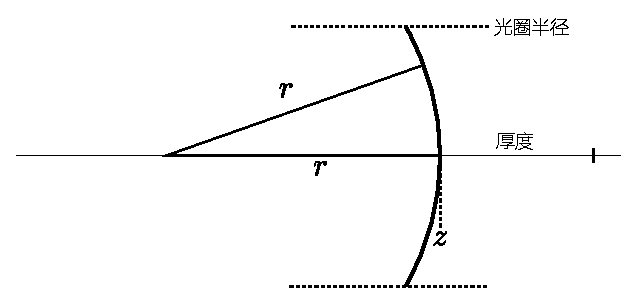
\includegraphics[width=0.6\linewidth]{chap06/Lenselement.eps}
    \caption{透镜界面(实曲线)与光轴相交于位置$z$。界面几何形状由
        表示其在光轴上下方范围的光圈半径以及元件的曲率半径$r$描述。
        如果元件有球形横截面,则它的轮廓由球心在光轴上距离$r$的球体给定,
        该球体也穿过$z$。如果$r$是负的,则元件界面就如从场景中看到那样是凹的
        (如图所示);否则就是\protect\keyindex{凸}{convex}{}的。透镜厚度给出了到
        右边下一个界面的距离,或者对于最右边的界面是到胶片平面的距离。}
    \label{fig:6.17}
\end{figure}

结构体\refvar{LensElementInterface}{}表示单个透镜元件界面。
\begin{lstlisting}
`\initcode{RealisticCamera Private Declarations}{=}`
struct `\initvar{LensElementInterface}{}` {
    `\refvar{Float}{}` `\initvar{curvatureRadius}{}`;
    `\refvar{Float}{}` `\initvar{thickness}{}`;
    `\refvar{Float}{}` `\initvar[LensElementInterface::eta]{eta}{}`;
    `\refvar{Float}{}` `\initvar{apertureRadius}{}`;
};
\end{lstlisting}

这里没有介绍的代码片\refcode{Load element data from lens description file}{}
\sidenote{译者注:我补充回来了。}读取透镜元件
并初始化数组\refvar[elementInterfaces]{RealisticCamera::elementInterfaces}{}。
见源代码中的注释了解该文件格式的细节,它并行化\reftab{6.1}中的结构,
并见pbrt发行版中的目录{\ttfamily scenes/lenses}了解大量透镜描述示例。

对从文件读取的值做了两个调整:第一,透镜系统传统上用毫米单位描述,
但pbrt假设场景单位用米。因此,除了折射率外的域都按1/1000缩小。
第二,元件直径被除以二;在下面的代码中半径是用起来更方便的量。
\begin{lstlisting}
`\refcode{RealisticCamera Private Data}{+=}\lastnext{RealisticCameraPrivateData}`
std::vector<`\refvar{LensElementInterface}{}`> `\initvar{elementInterfaces}{}`;
\end{lstlisting}

一旦加载完透镜界面描述,让一些关于透镜系统的值随时可得是很有用的。
\refvar{LensRearZ}{()}和\refvar{LensFrontZ}{()}分别返回
透镜系统尾部和头部元件的$z$深度。注意返回的$z$深度在相机空间中,
而不是透镜空间中,所以为正值。
\begin{lstlisting}
`\initcode{RealisticCamera Private Methods}{=}\initnext{RealisticCameraPrivateMethods}`
`\refvar{Float}{}` `\initvar{LensRearZ}{}`() const {
    return `\refvar{elementInterfaces}{}`.back().`\refvar{thickness}{}`;
}
\end{lstlisting}

求头部元件$z$位置需要求所有元件厚度之和(见\reffig{6.18})。
任何位于系统性能敏感部分的代码都不需要该值,
所以在需要时重算它就行。如果该方法对性能有影响,
最好还是在\refvar{RealisticCamera}{}中缓存该值。
\begin{figure}[htbp]
    \centering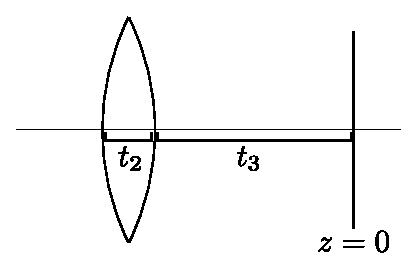
\includegraphics[width=0.4\linewidth]{chap06/Elementthicknessandposition.eps}
    \caption{元件厚度与光轴上位置的关系。胶片平面位于$z=0$,尾部元件的厚度$t_3$给出
        了从胶片到其界面的距离;这里尾部界面与轴交于$z=-t_3$。下一个元件厚度为$t_2$且
        位于$z=-t_3-t_2$,以此类推。头部元件交$z$轴于$\sum_i-t_i$。}
    \label{fig:6.18}
\end{figure}
\begin{lstlisting}
`\refcode{RealisticCamera Private Methods}{+=}\lastnext{RealisticCameraPrivateMethods}`
`\refvar{Float}{}` `\initvar{LensFrontZ}{}`() const {
    `\refvar{Float}{}` zSum = 0;
    for (const `\refvar{LensElementInterface}{}` &element : `\refvar{elementInterfaces}{}`)
        zSum += element.`\refvar{thickness}{}`;
    return zSum;
}
\end{lstlisting}

\refvar{RearElementRadius}{()}按单位米返回尾部元件光圈半径。
\begin{lstlisting}
`\refcode{RealisticCamera Private Methods}{+=}\lastnext{RealisticCameraPrivateMethods}`
`\refvar{Float}{}` `\initvar{RearElementRadius}{}`() const {
    return `\refvar{elementInterfaces}{}`.back().`\refvar{apertureRadius}{}`;
}
\end{lstlisting}
\subsection{追踪穿过透镜的光线}\label{sub:追踪穿过透镜的光线}
给定起始于透镜系统胶片一侧的光线,\refvar{TraceLensesFromFilm}{()}依次
计算与每个元件的相交处,如果其路径在穿过透镜系统途中被挡住了就终结该光线并返回{\ttfamily false}。
否则它就返回{\ttfamily true}并用相机空间中退出的光线来初始化{\ttfamily *rOut}。
在遍历时,{\ttfamily elementZ}追踪当前透镜元件的$z$截距。
因为光线起始于胶片,所以按照和\refvar{elementInterfaces}{}存储的相反顺序遍历透镜。
\begin{lstlisting}
`\refcode{RealisticCamera Method Definitions}{+=}\lastnext{RealisticCameraMethodDefinitions}`
bool `\refvar{RealisticCamera}{}`::`\initvar{TraceLensesFromFilm}{}`(const `\refvar{Ray}{}` &rCamera,
        `\refvar{Ray}{}` *rOut) const {
    `\refvar{Float}{}` elementZ = 0;
    `\refcode{Transform rCamera from camera to lens system space}{}`
    for (int i = `\refvar{elementInterfaces}{}`.size() - 1; i >= 0; --i) {
        const `\refvar{LensElementInterface}{}` &element = `\refvar{elementInterfaces}{}`[i];
        `\refcode{Update ray from film accounting for interaction with element}{}`
    }
    `\refcode{Transform rLens from lens system space back to camera space}{}`
    return true;
}
\end{lstlisting}

因为在pbrt的相机空间中相机指向$+z$轴但透镜在$-z$轴,
所以射线端点和方向的$z$分量需要取反。
尽管这是个简单到可以直接施加的变换,
我们还是偏好用显式的\refvar{Transform}{}使目的更明确。
\begin{lstlisting}
`\initcode{Transform rCamera from camera to lens system space}{=}`
static const `\refvar{Transform}{}` CameraToLens = `\refvar{Scale}{}`(1, 1, -1);
`\refvar{Ray}{}` rLens = CameraToLens(rCamera);
\end{lstlisting}

回想\reffig{6.18}中怎样计算元件的$z$截距:
因为我们从后往前访问元件,所以在考虑该元件的作用前
必须从{\ttfamily elementZ}中减去元件的厚度来计算其$z$截距。
\begin{lstlisting}
`\initcode{Update ray from film accounting for interaction with element}{=}`
elementZ -= element.`\refvar{thickness}{}`;
`\refcode{Compute intersection of ray with lens element}{}`
`\refcode{Test intersection point against element aperture}{}`
`\refcode{Update ray path for element interface interaction}{}`
\end{lstlisting}

有了元件的$z$轴截距,下一步是计算沿光线与元件界面(或光圈平面)相交处的参数值$t$。
对于光圈,采用光线-平面测试(见\refsub{光线-边界相交})。
对于球形界面,\refvar{IntersectSphericalElement}{()}执行该测试
并且如果找到相交处则还返回曲面法线;计算折射光方向时将需要该法线。
\begin{lstlisting}
`\initcode{Compute intersection of ray with lens element}{=}`
`\refvar{Float}{}` t;
`\refvar{Normal3f}{}` n;
bool isStop = (element.`\refvar{curvatureRadius}{}` == 0);
if (isStop)
    t = (elementZ - rLens.`\refvar[Ray::o]{o}{}`.z) / rLens.`\refvar[Ray::d]{d}{}`.z;
else {
    `\refvar{Float}{}` radius = element.`\refvar{curvatureRadius}{}`;
    `\refvar{Float}{}` zCenter = elementZ + element.`\refvar{curvatureRadius}{}`;
    if (!`\refvar{IntersectSphericalElement}{}`(radius, zCenter, rLens, &t, &n))
        return false;
}
\end{lstlisting}

方法\refvar{IntersectSphericalElement}{()}大致
和\refvar{Sphere::Intersect}{()}一样,不过它专门针对
元件中心在$z$轴上(且因此中心的$x$和$y$分量为零)这一情况。
这里文中没有包含代码片\refcode{Compute t0 and t1 for ray-element intersection}{}
和\refcode{Compute surface normal of element at ray intersection point}{},因为它们和
\refvar{Sphere::Intersect}{()}的实现一样\sidenote{译者注:我补充回来了。}。
\begin{lstlisting}
`\refcode{RealisticCamera Method Definitions}{+=}\lastnext{RealisticCameraMethodDefinitions}`
bool `\refvar{RealisticCamera}{}`::`\initvar{IntersectSphericalElement}{}`(`\refvar{Float}{}` radius,
        `\refvar{Float}{}` zCenter, const `\refvar{Ray}{}` &ray, `\refvar{Float}{}` *t, `\refvar{Normal3f}{}` *n) {
    `\refcode{Compute t0 and t1 for ray-element intersection}{}`
    `\refcode{Select intersection  based on ray direction and element curvature}{}`
    `\refcode{Compute surface normal of element at ray intersection point}{}`
    return true;
}
\end{lstlisting}
\begin{lstlisting}
`\initcode{Compute t0 and t1 for ray-element intersection}{=}`
`\refvar{Point3f}{}` o = ray.`\refvar[Ray::o]{o}{}` - `\refvar{Vector3f}{}`(0, 0, zCenter);
`\refvar{Float}{}` A = ray.`\refvar[Ray::d]{d}{}`.x*ray.`\refvar[Ray::d]{d}{}`.x + ray.`\refvar[Ray::d]{d}{}`.y*ray.`\refvar[Ray::d]{d}{}`.y + ray.`\refvar[Ray::d]{d}{}`.z*ray.`\refvar[Ray::d]{d}{}`.z;
`\refvar{Float}{}` B = 2 * (ray.`\refvar[Ray::d]{d}{}`.x*o.x + ray.`\refvar[Ray::d]{d}{}`.y*o.y + ray.`\refvar[Ray::d]{d}{}`.z*o.z);
`\refvar{Float}{}` C = o.x*o.x + o.y*o.y + o.z*o.z - radius*radius;
`\refvar{Float}{}` t0, t1;
if (!`\refvar{Quadratic}{}`(A, B, C, &t0, &t1))
    return false;
\end{lstlisting}
\begin{lstlisting}
`\initcode{Compute surface normal of element at ray intersection point}{=}`
*n = `\refvar{Normal3f}{}`(`\refvar{Vector3f}{}`(o + *t * ray.`\refvar[Ray::d]{d}{}`));
*n = `\refvar{Faceforward}{}`(`\refvar{Normalize}{}`(*n), -ray.`\refvar[Ray::d]{d}{}`);
\end{lstlisting}

然而这里在选择返回哪个交点时有个微妙之处\sidenote{译者注:原文subtlety。}:
$t>0$的最近相交处不一定在元件界面上;
见\reffig{6.19}\footnote{“微妙之处”(subtlety)一般意味着作者花费好几个小时来调试它。}。
例如,对于自场景中接近并与(具有负曲率半径的)凹透镜相交的光线,
两个相交处中不管近处那个是否有$t>0$都该返回远处那个。
幸运的是,基于光线方向和曲率半径的简单逻辑可指明用哪个$t$值。
\begin{figure}[htbp]
    \centering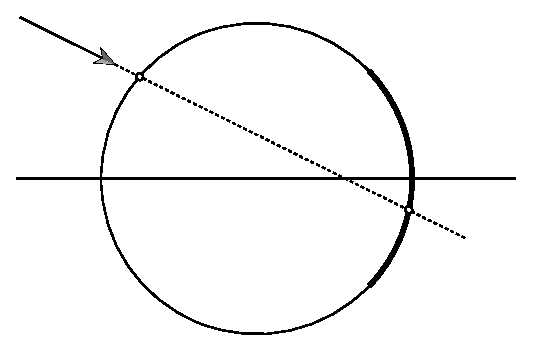
\includegraphics[width=0.5\linewidth]{chap06/Lenscorrectintersection.eps}
    \caption{当计算光线与球形透镜元件的相交处时,光线与整球的首个相交处不一定是我们想要的。
        这里,第二个相交处才在真正的元件界面(粗线)上,而第一个应该被忽略。}
    \label{fig:6.19}
\end{figure}
\begin{lstlisting}
`\initcode{Select intersection  based on ray direction and element curvature}{=}`
bool useCloserT = (ray.`\refvar[Ray::d]{d}{}`.z > 0) ^ (radius < 0);
*t = useCloserT ? std::min(t0, t1) : std::max(t0, t1);
if (*t < 0)
    return false;
\end{lstlisting}

每个透镜元件都按某半径绕光轴扩展;如果与该元件的交点在该半径之外,
则该光线实际上将与镜头罩相交并终止。
类似地,如果光线与光圈相交,它也会终止。
因此,这里我们用当前元件的适用限制来测试交点,
要么终止该光线,要么它幸存下来并将其端点更新为当前交点。
\begin{lstlisting}
`\initcode{Test intersection point against element aperture}{=}`
`\refvar{Point3f}{}` pHit = rLens(t);
`\refvar{Float}{}` r2 = pHit.x * pHit.x + pHit.y * pHit.y;
if (r2 > element.`\refvar{apertureRadius}{}` * element.`\refvar{apertureRadius}{}`)
    return false;
rLens.`\refvar[Ray::o]{o}{}` = pHit;
\end{lstlisting}

如果当前元件是光圈,则光路在穿过元件界面时不受影响。
对于玻璃(或塑料)透镜元件,光线在从具有某个折射率的介质进入
到具有另一折射率的介质时在交界面会改变方向
(光线可能从空气进入玻璃、从玻璃进入空气,或者从
具有某个折射率的玻璃进入具有不同折射率的另一种玻璃)。

\refsec{镜面反射与透射}讨论了两种介质边界间折射率的变化
将怎样改变光线的方向及其携带的辐射量(这里的情况下
我们可以忽略辐射量的变化,因为如果光线在进入和退出透镜系统时
处于同一种介质中则这种效应会抵消掉——这里都是空气)。
函数\refvar{Refract}{()}定义在\refsub{镜面透射};
注意它预设入射方向指向远离曲面的方向,所以传入前要对光线方向取反。
该函数在出现\keyindex{全内反射}{total internal reflection}{reflection反射}时
返回{\ttfamily false},该情况下光路终止。
否则在{\ttfamily w}中返回折射方向。

通常,穿过这类界面时一些光被透射而另一些被反射。
这里我们忽略反射并假设完美传输。尽管这是种近似,但它是合理的:
制造透镜时一般用了设计的涂料把反射降低到光线所带辐射的0.25\%左右
(然而,对这少量的反射建模对于实现\keyindex{镜头光晕}{lens flare}{}会很重要)。
\begin{lstlisting}
`\initcode{Update ray path for element interface interaction}{=}`
if (!isStop) {
    `\refvar{Vector3f}{}` w;
    `\refvar{Float}{}` etaI = element.`\refvar[LensElementInterface::eta]{eta}{}`;
    `\refvar{Float}{}` etaT = (i > 0 && `\refvar{elementInterfaces}{}`[i - 1].`\refvar[LensElementInterface::eta]{eta}{}` != 0) ?
        `\refvar{elementInterfaces}{}`[i - 1].`\refvar[LensElementInterface::eta]{eta}{}` : 1;
    if (!`\refvar{Refract}{}`(`\refvar{Normalize}{}`(-rLens.`\refvar[Ray::d]{d}{}`), n, etaI / etaT, &w))
        return false;
    rLens.`\refvar[Ray::d]{d}{}` = w;
}
\end{lstlisting}

若光线成功从前端透镜元件射出,它只需要从透镜空间变换到相机空间。
\begin{lstlisting}
`\initcode{Transform rLens from lens system space back to camera space}{=}`
if (rOut != nullptr) {
    static const `\refvar{Transform}{}` LensToCamera = `\refvar{Scale}{}`(1, 1, -1);
    *rOut = LensToCamera(rLens);
}
\end{lstlisting}

方法\refvar{TraceLensesFromScene}{()}和\refvar{TraceLensesFromFilm}{()}非常相似,这里不再介绍。
主要差别在于它是从前往后而不是从后往前遍历元件。
注意它假设传入的光线已经在相机空间了;
如果光线始于世界空间则调用者应负责执行该变换。
返回的光线位于尾部透镜元件朝向胶片的相机空间中。
\begin{lstlisting}
`\refcode{RealisticCamera Private Methods}{+=}\lastcode{RealisticCameraPrivateMethods}`
bool `\initvar{TraceLensesFromScene}{}`(const `\refvar{Ray}{}` &rCamera, `\refvar{Ray}{}` *rOut) const;
\end{lstlisting}

\subsection{厚透镜近似}\label{sub:厚透镜近似}
\refsub{薄透镜模型与景深}中用的薄透镜近似是基于透镜系统沿光轴厚度为0的简化假设。
透镜系统的厚透镜近似因为考虑了透镜系统的$z$范围而更精确些。
这里在介绍厚透镜的基本概念之后,我们将用厚透镜近似来确定
要把透镜系统放在离胶片多远处来对焦\refsub{对焦}中想要的对焦深度。

厚透镜近似将透镜系统表示为两对沿光轴的距离——
\keyindex{焦点}{focal point}{}以及\keyindex{主平面}{principal plane}{};
一个透镜系统有两个\keyindex{主点}{cardinal point}{}。
如果经由一个理想透镜系统追踪平行于光轴的光线,
则所有这些光线将会交于光轴上同一点——这就是焦点
(实际中,真实透镜系统并不绝对理想,不同高度的入射光线
与光轴将相交于一个$z$值小范围——这就是\keyindex{球面像差}{spherical aberration}{})。
有了特定的透镜系统,我们就能从每一侧追踪穿过它且与光轴平行的光线,
并计算它们与$z$轴的相交处以找到焦点(见\reffig{6.20})。
\begin{figure}[htbp]
    \centering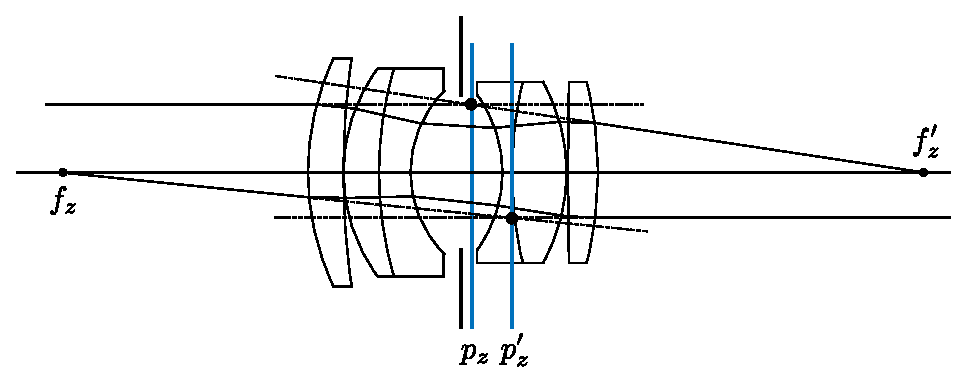
\includegraphics[width=\linewidth]{chap06/Lenssystemcardinalpoints.eps}
    \caption{计算透镜系统的主点。文件{\ttfamily lenses/dgauss.dat}中
    描述的透镜系统,来自场景的入射光线平行于光轴(轴上方),
    来自胶片的光线平行于光轴(下方)。这些入射光线对应的
    离开透镜系统的光线与光轴的相交处给出了两个焦点$f'_z$(胶片一侧)
    和$f_z$(场景一侧)。每对入射和出射光线的延长线以及原始光线的相交处给定了
    主平面$z=p_z$和$z=p'_z$,这里表示为垂直于光轴的蓝线。}
    \label{fig:6.20}
\end{figure}

每个主平面通过延长平行于光轴的入射光线以及离开透镜的光线直至相交来求得;
相交处的$z$深度给出了对应主平面的深度。\reffig{6.20}展示了
一个透镜系统及其焦点$f_z$和$f'_z$以及位于$z$值$p_z$和$p'_z$的主平面
(正如\refsub{薄透镜模型与景深},有撇的变量表示透镜系统胶片一侧的点,
无撇的变量表示场景中要成像的点)。

给定离开透镜的光线,求焦点要先计算光线的$x$和$y$分量为零时的值$t_{\mathrm{f}}$。
若进入的光线只沿$x$偏移了光轴,则我们要求出
使$o_x+t_{\mathrm{f}}d_x=0$的$t_{\mathrm{f}}$。因此
\begin{align*}
    t_{\mathrm{f}}=\frac{-o_x}{d_x}\, .
\end{align*}
同样的方法,为了求得离开透镜的光线与原始光线有相同高度处
的主平面的$t_{\mathrm{p}}$,我们有$o_x+t_{\mathrm{p}}d_x=x$,因此
\begin{align*}
    t_{\mathrm{p}}=\frac{x-o_x}{d_x}\, .
\end{align*}
一旦算出这两个$t$值,射线方程就可用于求得对应点的$z$坐标。

方法\refvar{ComputeCardinalPoints}{()}为给定光线计算焦点和主平面的$z$深度。
注意它假设光线在相机空间中但返回透镜空间中沿光轴的$z$值。
\begin{lstlisting}
`\refcode{RealisticCamera Method Definitions}{+=}\lastnext{RealisticCameraMethodDefinitions}`
void `\refvar{RealisticCamera}{}`::`\initvar{ComputeCardinalPoints}{}`(const `\refvar{Ray}{}` &rIn,
        const `\refvar{Ray}{}` &rOut, `\refvar{Float}{}` *pz, `\refvar{Float}{}` *fz) {
    `\refvar{Float}{}` tf = -rOut.`\refvar[Ray::o]{o}{}`.x / rOut.`\refvar[Ray::d]{d}{}`.x;
    *fz = -rOut(tf).z;
    `\refvar{Float}{}` tp = (rIn.`\refvar[Ray::o]{o}{}`.x - rOut.`\refvar[Ray::o]{o}{}`.x) / rOut.`\refvar[Ray::d]{d}{}`.x;
    *pz = -rOut(tp).z;
}
\end{lstlisting}

方法\refvar{ComputeThickLensApproximation}{()}为透镜系统
计算两对主点。
\begin{lstlisting}
`\refcode{RealisticCamera Method Definitions}{+=}\lastnext{RealisticCameraMethodDefinitions}`
void `\refvar{RealisticCamera}{}`::`\initvar{ComputeThickLensApproximation}{}`(`\refvar{Float}{}` pz[2],
        `\refvar{Float}{}` fz[2]) const {
    `\refcode{Find height x from optical axis for parallel rays}{}`
    `\refcode{Compute cardinal points for film side of lens system}{}`
    `\refcode{Compute cardinal points for scene side of lens system}{}`
}
\end{lstlisting}

首先,我们必须为追踪的光线选择沿$x$轴的高度。
它应该离$x=0$足够远使得有足够数值精度来准确计算
离开透镜系统的光线与$z$轴相交于哪里,
但$x$轴上也不能太高以免在光线穿过透镜系统时命中光圈。
这里,我们采用胶片对角范围的很小比例;其效果一般很好,除非光圈非常小。
\begin{lstlisting}
`\initcode{Find height x from optical axis for parallel rays}{=}`
`\refvar{Float}{}` x = .001 * `\refvar{film}{}`->`\refvar{diagonal}{}`;
\end{lstlisting}

为了构建从场景进入透镜系统的光线{\ttfamily rScene},
我们从透镜前端偏移一点(回想传入\refvar{TraceLensesFromScene}{()}的
光线应该在相机空间)。
\begin{lstlisting}
`\initcode{Compute cardinal points for film side of lens system}{=}`
`\refvar{Ray}{}` rScene(`\refvar{Point3f}{}`(x, 0, `\refvar{LensFrontZ}{}`() + 1), `\refvar{Vector3f}{}`(0, 0, -1));
`\refvar{Ray}{}` rFilm;
`\refvar{TraceLensesFromScene}{}`(rScene, &rFilm);
`\refvar{ComputeCardinalPoints}{}`(rScene, rFilm, &pz[0], &fz[0]);
\end{lstlisting}

从透镜系统胶片一侧起始的等价过程为我们给出了另外两个主点。
\begin{lstlisting}
`\initcode{Compute cardinal points for scene side of lens system}{=}`
rFilm = `\refvar{Ray}{}`(`\refvar{Point3f}{}`(x, 0, `\refvar{LensRearZ}{}`() - 1), `\refvar{Vector3f}{}`(0, 0, 1));
`\refvar{TraceLensesFromFilm}{}`(rFilm, &rScene);
`\refvar{ComputeCardinalPoints}{}`(rFilm, rScene, &pz[1], &fz[1]);
\end{lstlisting}

\subsection{对焦}\label{sub:对焦}
透镜系统可以通过相对于胶片移动来对焦场景中的指定深度,
这样在想要的对焦深度处的点成像为胶片平面上的一点。
高斯透镜方程\refeq{6.3}给了我们一个可解的关系来对焦厚透镜。

对于厚透镜,高斯透镜方程把到场景中位于$z$处的点的距离
和它对焦到$z'$的点用下式联系起来:
\begin{align}\label{eq:6.3}
    \frac{1}{z'-p'_z}-\frac{1}{z-p_z}=\frac{1}{f}\, .
\end{align}
对于薄透镜,$p_z=p'_z=0$,即推出\refeq{6.1}。

如果我们知道主平面的位置$p_z$和$p'_z$以及透镜的焦距$f$
并想要对焦沿光轴的某个深度$z$,则我们需确定应将系统平移多远$\delta$使得
\begin{align*}
    \frac{1}{z'-p'_z+\delta}-\frac{1}{z-p_z+\delta}=\frac{1}{f}\, .
\end{align*}

胶片一侧的焦点应在胶片上,所以$z'=0$,且$z=z_{\mathrm{f}}$即给定的对焦深度。
唯一未知的是$\delta$,一些代数处理为我们给出
\begin{align}\label{eq:6.4}
    \delta=\frac{1}{2}\left(p_z-z_{\mathrm{f}}+p'_z-\sqrt{(p_z-z_{\mathrm{f}}-p'_z)(p_z-z_{\mathrm{f}}-4f-p'_z)}\right)\, .
\end{align}
(实际上有两个解,但两个中更近的这个解给出了对透镜位置较小的调整,因此是合适的那个。)

\refvar{FocusThickLens}{()}用该近似对焦透镜系统。
计算$\delta$后,它返回应放置透镜系统处沿$z$轴离胶片的偏移量。
\begin{lstlisting}
`\refcode{RealisticCamera Method Definitions}{+=}\lastnext{RealisticCameraMethodDefinitions}`
`\refvar{Float}{}` `\refvar{RealisticCamera}{}`::`\initvar{FocusThickLens}{}`(`\refvar{Float}{}` focusDistance) {
    `\refvar{Float}{}` pz[2], fz[2];
    `\refvar{ComputeThickLensApproximation}{}`(pz, fz);
    `\refcode{Compute translation of lens, delta, to focus at focusDistance}{}`
    return `\refvar{elementInterfaces}{}`.back().`\refvar{thickness}{}` + delta;
}
\end{lstlisting}

\refeq{6.4}给出了偏移量$\delta$。透镜的焦距$f$是主点$f'_z$和$p'_z$间的距离。
还要注意对于$z$用的是对焦距离的相反数,因为光轴指向负的$z$。
\begin{lstlisting}
`\initcode{Compute translation of lens, delta, to focus at focusDistance}{=}`
`\refvar{Float}{}` f = fz[0] - pz[0];
`\refvar{Float}{}` z = -focusDistance;
`\refvar{Float}{}` delta = 0.5f * (pz[1] - z + pz[0] -
    std::sqrt((pz[1] - z - pz[0]) * (pz[1] - z - 4 * f - pz[0])));
\end{lstlisting}

我们现在终于可以实现\refvar{RealisticCamera}{}构造函数中
对焦透镜系统的代码片了(回想最尾部元件界面的厚度是该界面到胶片的距离)。
\begin{lstlisting}
`\initcode{Compute lens-film distance for given focus distance}{=}`
`\refvar{elementInterfaces}{}`.back().`\refvar{thickness}{}` = `\refvar{FocusThickLens}{}`(focusDistance);
\end{lstlisting}

\subsection{出射瞳}\label{sub:出射瞳}
不是所有从胶片平面上给定点起始朝向尾部透镜元件的光线都能成功射出透镜系统;
一些会被光圈阻挡或者与透镜系统外壳相交。
反过来,尾部透镜元件上不是所有点都能把辐射传输到胶片上的点。
尾部元件上确实能带着光通过透镜系统的点集称为\keyindex{出射瞳}{exit pupil}{};
它的尺寸和位置随着胶片平面上的视点变化
(类似地,\keyindex{入射瞳}{entrance pupil}{}是场景中给定点起始
且能到达胶片的光线所穿过的前端透镜元件区域)。

\reffig{6.21}展示了广角镜头从胶片平面上两点看到的出射瞳。
当点靠近胶片边缘时出射瞳更小。这类收缩的一个结果是暗角。
\begin{figure}[htbp]
    \centering
    \subfloat[]{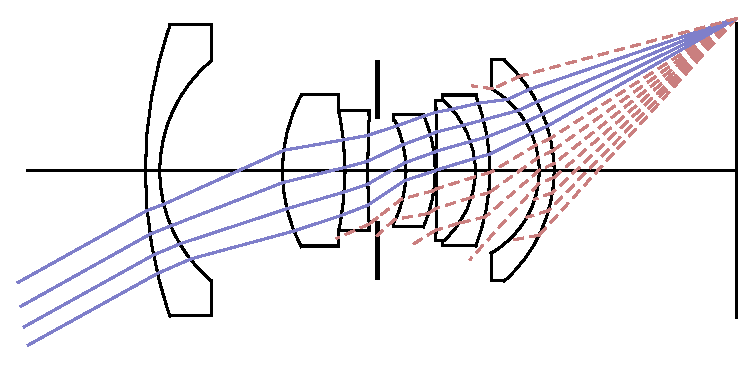
\includegraphics[width=0.5\linewidth]{chap06/wide22-rays-edge.eps}\label{fig:6.21.1}}\qquad
    \subfloat[]{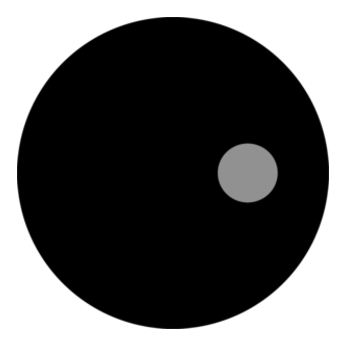
\includegraphics[width=0.2\linewidth]{chap06/wide22-exit-edge.eps}\label{fig:6.21.2}}\\
    \subfloat[]{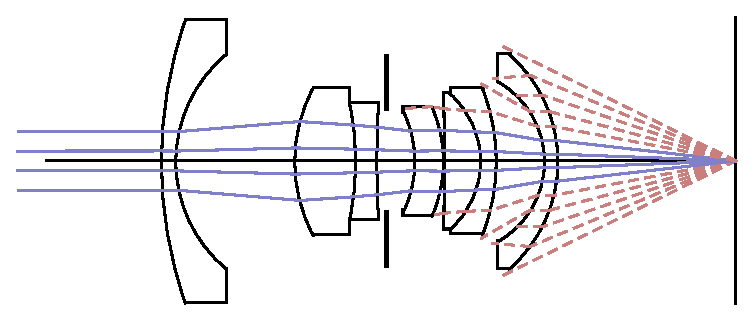
\includegraphics[width=0.5\linewidth]{chap06/wide22-rays-middle.eps}\label{fig:6.21.3}}\qquad
    \subfloat[]{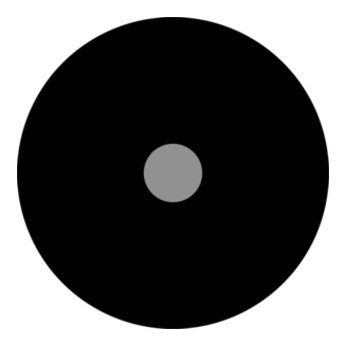
\includegraphics[width=0.2\linewidth]{chap06/wide22-exit-middle.eps}\label{fig:6.21.4}}
    \caption{22mm广角镜头在5.5mm光圈(f/4)下的出射瞳。
        (a)起始于胶片平面边缘一点的光线进入尾部透镜元件的多个点。
        虚线表示被阻挡而没有射出透镜系统的光线。
        (b)从(a)中的有利位置看到的出射瞳的像。尾部透镜元件是黑色的,而出射瞳表示为灰色。
        (c)在胶片中心,不同的出射瞳区域允许光线射出到场景中。
        (d)从胶片中心看到的出射瞳的像。}
    \label{fig:6.21}
\end{figure}

当追踪起始于胶片的光线时,我们想避免追踪太多没能穿过透镜系统的光线;
因此值得把采样限制在出射瞳本身及其周围很小区域内,
而不是浪费地在尾部透镜元件整个区域上采样。

在追踪光线前计算胶片上每点的出射瞳会开销极大;相反\refvar{RealisticCamera}{}
的实现预先计算沿胶片平面上的直线段对应的出射瞳边界。
因为我们假设透镜系统是绕光轴径向对称的,所以出射瞳边界也会是径向对称的,
且胶片平面上任意点的边界都可以通过适当旋转这些线段边界来求得(\reffig{6.22})
\sidenote{译者注:\protect\reffig{6.22}题注最后一句翻译不确定是否正确。}。
然后这些边界用于为特定胶片采样位置高效求取出射瞳边界。
\begin{figure}[htbp]
    \centering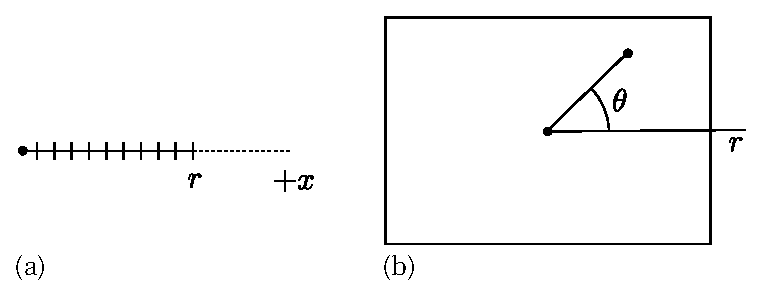
\includegraphics[width=0.7\linewidth]{chap06/Exitpupilboundsfilm.eps}
    \caption{预先计算出射瞳边界。(a)\refvar{RealisticCamera}{}为胶片平面上
        沿$x$轴的一系列线段计算出射瞳的边界,直到胶片中心到角点的距离$r$。
        (b)鉴于径向对称的假设,我们可以通过计算点与$x$轴间的夹角$\theta$来
        为胶片上的任意点(实心点)求取出射瞳边界。如果原始出射瞳边界内的一点被采样
        再旋转$\theta$,则我们就有了原始点处出射瞳内的一点。}
    \label{fig:6.22}
\end{figure}

需要意识到的一个重要细节是,由于透镜系统通过沿光轴平移来对焦,
所以当调整透镜系统的对焦时出射瞳的形状和位置会变化。
因此在对焦后才计算这些边界十分重要
\footnote{作者也是调试几个小时后才痛苦地吸取这一教训。}。
\begin{lstlisting}
`\initcode{Compute exit pupil bounds at sampled points on the film}{=}`
int nSamples = 64;
`\refvar{exitPupilBounds}{}`.resize(nSamples);
`\refvar{ParallelFor}{}`(
    [&](int i) {
        `\refvar{Float}{}` r0 = (`\refvar{Float}{}`)i / nSamples * `\refvar{film}{}`->`\refvar{diagonal}{}` / 2;
        `\refvar{Float}{}` r1 = (`\refvar{Float}{}`)(i + 1) / nSamples * `\refvar{film}{}`->`\refvar{diagonal}{}` / 2;
        `\refvar{exitPupilBounds}{}`[i] = `\refvar{BoundExitPupil}{}`(r0, r1);
    }, nSamples);
\end{lstlisting}
\begin{lstlisting}
`\refcode{RealisticCamera Private Data}{+=}\lastcode{RealisticCameraPrivateData}`
std::vector<`\refvar{Bounds2f}{}`> `\initvar{exitPupilBounds}{}`;
\end{lstlisting}

方法\refvar{BoundExitPupil}{()}计算从胶片平面上一段点看到的出射瞳2D边界框。
通过尝试追踪在尾部透镜元件切平面的一组点上穿过透镜系统的光线来求取该边界框。
成功穿过透镜系统的光线的边界框便给出了出射瞳的大致边界——见\reffig{6.23}。
\begin{figure}[htbp]
    \centering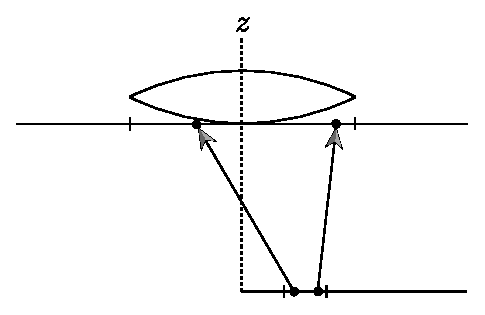
\includegraphics[width=0.5\linewidth]{chap06/Sampleexitpupil.eps}
    \caption{怎样计算出射瞳边界的2D图示。\refvar{BoundExitPupil}{()}接收
        胶片上沿$x$轴的区间。它沿区间采样一系列点(图中下方)。
        对于每个点,它还采样尾部透镜元件在与其尾部相切的平面上对应范围的边框内的一点。
        它计算所有起始于区间的点且成功穿过透镜系统的光线在切平面上的边界框。}
    \label{fig:6.23}
\end{figure}
\begin{lstlisting}
`\refcode{RealisticCamera Method Definitions}{+=}\lastnext{RealisticCameraMethodDefinitions}`
`\refvar{Bounds2f}{}` `\refvar{RealisticCamera}{}`::`\initvar{BoundExitPupil}{}`(`\refvar{Float}{}` pFilmX0,
        `\refvar{Float}{}` pFilmX1) const {
    `\refvar{Bounds2f}{}` pupilBounds;
    `\refcode{Sample a collection of points on the rear lens to find exit pupil}{}`
    `\refcode{Return entire element bounds if no rays made it through the lens system}{}`
    `\refcode{Expand bounds to account for sample spacing}{}`
    return pupilBounds;
}
\end{lstlisting}

该实现非常密集地采样出射瞳——每段共有$1024^2$个点。
我们发现实践中该采样率能提供很好的出射瞳边界。
\begin{lstlisting}
`\initcode{Sample a collection of points on the rear lens to find exit pupil}{=}`
const int nSamples = 1024 * 1024;
int nExitingRays = 0;
`\refcode{Compute bounding box of projection of rear element on sampling plane}{}`
for (int i = 0; i < nSamples; ++i) {
    `\refcode{Find location of sample points on x segment and rear lens element}{}`
    `\refcode{Expand pupil bounds if ray makes it through the lens system}{}`
}
\end{lstlisting}

尾部元件在与之垂直的平面上的边界框不足以成为出射瞳在该平面上的投影的保守边界框;
因为元件一般是曲形的,穿过该平面边界之外的光线可能自己与尾部透镜元件有效范围相交。
比起计算精确边界,我们则是大幅增大边框。结果是用来计算出射瞳边界而采样的许多点会被浪费;
实践中,这是很小的代价,因为通常这些样本在透镜的光线追踪阶段会很快被终止。
\begin{lstlisting}
`\initcode{Compute bounding box of projection of rear element on sampling plane}{=}`
`\refvar{Float}{}` rearRadius = `\refvar{RearElementRadius}{}`();
`\refvar{Bounds2f}{}` projRearBounds(`\refvar{Point2f}{}`(-1.5f * rearRadius, -1.5f * rearRadius),
                        `\refvar{Point2f}{}`( 1.5f * rearRadius,  1.5f * rearRadius));
\end{lstlisting}

通过在$x$区间端点间线性插值来求得胶片上的$x$样本点。
稍后\refsub{Hammersley和Halton序列}{}定义的函数\refvar{RadicalInverse}{()}用于
为出射瞳边界框内的采样点计算插值偏移量。我们将看到
这里实现的采样策略对应于在3D中使用Hammersley点;
得到的点集会最小化整个3D域覆盖情况的差异,反过来保证了准确估计出射瞳边界。
\begin{lstlisting}
`\initcode{Find location of sample points on x segment and rear lens element}{=}`
`\refvar{Point3f}{}` pFilm(`\refvar{Lerp}{}`((i + 0.5f) / nSamples, pFilmX0, pFilmX1), 0, 0);
`\refvar{Float}{}` u[2] = { `\refvar{RadicalInverse}{}`(0, i), `\refvar{RadicalInverse}{}`(1, i) };
`\refvar{Point3f}{}` pRear(`\refvar{Lerp}{}`(u[0], projRearBounds.pMin.x, projRearBounds.pMax.x),
              `\refvar{Lerp}{}`(u[1], projRearBounds.pMin.y, projRearBounds.pMax.y),
              `\refvar{LensRearZ}{}`());
\end{lstlisting}

现在我们可构造从{\ttfamily pFilm}到{\ttfamily pRear}的光线并
通过看它是否成功射出透镜系统前端来确定它是否在出射瞳内。
如果是,则拓展出射瞳边界以包含该点。如果采样点已经在
目前算出的出射瞳边界框内,则我们可以跳过光线追踪步骤以节约些无用功。
\begin{lstlisting}
`\initcode{Expand pupil bounds if ray makes it through the lens system}{=}`
if (`\refvar{Inside}{}`(`\refvar{Point2f}{}`(pRear.x, pRear.y), pupilBounds) ||
    `\refvar{TraceLensesFromFilm}{}`(`\refvar{Ray}{}`(pFilm, pRear - pFilm), nullptr)) {
    pupilBounds = `\refvar[Union1]{Union}{}`(pupilBounds, `\refvar{Point2f}{}`(pRear.x, pRear.y));
    ++nExitingRays;
}
\end{lstlisting}

可能没有样本光线能成功穿过透镜系统;例如一些在胶片范围边缘处出射瞳会消失的
超大广角镜头完全可能发生这种情况。这种情况下边界并不重要,
\refvar{BoundExitPupil}{()}返回包括了整个尾部透镜元件的边界。
\begin{lstlisting}
`\initcode{Return entire element bounds if no rays made it through the lens system}{=}`
if (nExitingRays == 0) 
    return projRearBounds;
\end{lstlisting}

当一个样本成功穿过透镜系统而它的一个相邻样本没有时,
有可能与该邻居很相近的另一个样本实际上能成功穿过。
因此,最终边界在每个方向上再大致按样本间距拓展以考虑这一不确定性。
\begin{lstlisting}
`\initcode{Expand bounds to account for sample spacing}{=}`
pupilBounds = `\refvar{Expand}{}`(pupilBounds,
                     2 * projRearBounds.`\refvar{Diagonal}{}`().`\refvar{Length}{}`() /
                     std::sqrt(nSamples));
\end{lstlisting}

有了预先计算并存储在\refvar[exitPupilBounds]{RealisticCamera::exitPupilBounds}{}中的边界,
方法\refvar{SampleExitPupil}{()}就能很高效地为胶片平面上的给定点求得出射瞳边界。
为了准确地对成像辐射度量学建模,下列代码需要知道该边界框的面积,
所以它通过{\ttfamily sampleBoundsArea}返回。
\begin{lstlisting}
`\refcode{RealisticCamera Method Definitions}{+=}\lastnext{RealisticCameraMethodDefinitions}` 
`\refvar{Point3f}{}` `\refvar{RealisticCamera}{}`::`\initvar{SampleExitPupil}{}`(const `\refvar{Point2f}{}` &pFilm,
        const `\refvar{Point2f}{}` &lensSample, `\refvar{Float}{}` *sampleBoundsArea) const {
    `\refcode{Find exit pupil bound for sample distance from film center}{}`
    `\refcode{Generate sample point inside exit pupil bound}{}`
    `\refcode{Return sample point rotated by angle of pFilm with +x axis}{}`
}
\end{lstlisting}
\begin{lstlisting}
`\initcode{Find exit pupil bound for sample distance from film center}{=}`
`\refvar{Float}{}` rFilm = std::sqrt(pFilm.x * pFilm.x + pFilm.y * pFilm.y);
int rIndex = rFilm / (`\refvar{film}{}`->`\refvar{diagonal}{}` / 2) * `\refvar{exitPupilBounds}{}`.size();
rIndex = std::min((int)`\refvar{exitPupilBounds}{}`.size() - 1, rIndex);
`\refvar{Bounds2f}{}` pupilBounds = `\refvar{exitPupilBounds}{}`[rIndex];
if (sampleBoundsArea) *sampleBoundsArea = pupilBounds.Area();
\end{lstlisting}

给定瞳的边界框后,通过对提供的位于$[0,1)^2$的值{\ttfamily lensSample}线性插值
来采样边界框中的一点。
\begin{lstlisting}
`\initcode{Generate sample point inside exit pupil bound}{=}`
`\refvar{Point2f}{}` pLens = pupilBounds.`\refvar[Bounds3::Lerp]{Lerp}{}`(lensSample);
\end{lstlisting}

因为出射瞳边界是从胶片上一点沿$+x$轴算得的,
但点{\ttfamily pFilm}是胶片上的任意点,
故出射瞳边框内的样本点必须像{\ttfamily pFilm}对$+x$轴那样旋转相同角度。
\begin{lstlisting}
`\initcode{Return sample point rotated by angle of pFilm with +x axis}{=}`
`\refvar{Float}{}` sinTheta = (rFilm != 0) ? pFilm.y / rFilm : 0;
`\refvar{Float}{}` cosTheta = (rFilm != 0) ? pFilm.x / rFilm : 1;
return `\refvar{Point3f}{}`(cosTheta * pLens.x - sinTheta * pLens.y,
               sinTheta * pLens.x + cosTheta * pLens.y,
               `\refvar{LensRearZ}{}`());
\end{lstlisting}

\subsection{生成光线}\label{sub:生成光线}
现在我们有了机制去追踪穿过透镜系统的光线并采样由胶片平面上的点得来的出射瞳边界内的点,
将\refvar{CameraSample}{}转化为离开相机的光线非常简单:
我们需要计算样本在胶片平面上的位置并生成起始于该点射向尾部透镜元件的光线,
然后通过透镜系统追踪它。
\begin{lstlisting}
`\refcode{RealisticCamera Method Definitions}{+=}\lastcode{RealisticCameraMethodDefinitions}`
`\refvar{Float}{}` `\refvar{RealisticCamera}{}`::`\initvar[RealisticCamera::GenerateRay]{\refvar{GenerateRay}{}}{}`(const `\refvar{CameraSample}{}` &sample,
        `\refvar{Ray}{}` *ray) const {
    `\refcode{Find point on film, pFilm, corresponding to sample.pFilm}{}`
    `\refcode{Trace ray from pFilm through lens system}{}`
    `\refcode{Finish initialization of RealisticCamera ray}{}`
    `\refcode{Return weighting for RealisticCamera ray}{}`
}
\end{lstlisting}

值\refvar[pFilm]{CameraSample::pFilm}{}与图像的整个像素分辨率有关。
这里我们用传感器的物理模型来操作,所以我们开始先将样本转化回$[0,1)^2$中。
接着,通过用该样本值在其区域上线性插值来求得胶片上的对应点。
\begin{lstlisting}
`\initcode{Find point on film, pFilm, corresponding to sample.pFilm}{=}`
`\refvar{Point2f}{}` s(sample.`\refvar{pFilm}{}`.x / `\refvar{film}{}`->`\refvar{fullResolution}{}`.x,
          sample.`\refvar{pFilm}{}`.y / `\refvar{film}{}`->`\refvar{fullResolution}{}`.y);
`\refvar{Point2f}{}` pFilm2 = `\refvar{film}{}`->`\refvar{GetPhysicalExtent}{}`().`\refvar[Bounds3::Lerp]{Lerp}{}`(s);
`\refvar{Point2f}{}` pFilm(-pFilm2.x, pFilm2.y, 0);
\end{lstlisting}

然后\refvar{SampleExitPupil}{()}给我们尾部透镜元件切平面上的一点,
让我们确定了光线的方向。我们可追踪该光线穿过透镜系统。
若光线被光圈阻挡或没能成功穿过透镜系统,\refvar[RealisticCamera::GenerateRay]{GenerateRay}{()}返回权重0
(调用者应保证检查该情况)。
\begin{lstlisting}
`\initcode{Trace ray from pFilm through lens system}{=}`
`\refvar{Float}{}` exitPupilBoundsArea;
`\refvar{Point3f}{}` pRear = `\refvar{SampleExitPupil}{}`(`\refvar{Point2f}{}`(pFilm.x, pFilm.y), sample.`\refvar{pLens}{}`,
                                &exitPupilBoundsArea);
`\refvar{Ray}{}` rFilm(pFilm, pRear - pFilm, `\refvar{Infinity}{}`,
          `\refvar{Lerp}{}`(sample.`\refvar[CameraSample::time]{time}{}`, `\refvar{shutterOpen}{}`, `\refvar{shutterClose}{}`));
if (!`\refvar{TraceLensesFromFilm}{}`(rFilm, ray))
    return 0;
\end{lstlisting}

如果光线成功射出透镜系统,则需要处理常规细节以完成其初始化。
\begin{lstlisting}
`\initcode{Finish initialization of RealisticCamera ray}{=}`
*ray = `\refvar{CameraToWorld}{}`(*ray);
ray->`\refvar[Ray::d]{d}{}` = `\refvar{Normalize}{}`(ray->`\refvar[Ray::d]{d}{}`);
ray->`\refvar[Ray::medium]{medium}{}` = `\refvar[Camera::medium]{medium}{}`;
\end{lstlisting}

在介绍了蒙特卡洛积分一些必要的背景后,
代码片\refcode{Return weighting for RealisticCamera ray}{}将在\refsub{采样相机1}介绍。

\subsection{相机测量方程}\label{sub:相机测量方程}
有了上述对真实成像过程更精确的模拟,
更仔细地定义胶片或相机传感器的辐射度量是值得的。
从出射瞳到胶片的光线携带着来自场景的辐射;
因此从胶片平面上一点来考虑,有一组对应的辐射入射方向。
离开出射瞳的辐射分布会被胶片上该点所见的失焦模糊程度影响——
\reffig{6.24}展示了从胶片上两点看到的出射瞳辐射的渲染图。
\begin{figure}[htbp]
    \centering
    \includegraphics[width=0.4\linewidth]{chap06/exitpupil-a.png}\quad
    \includegraphics[width=0.4\linewidth]{chap06/exitpupil-b.png}
    \caption{从\reffig{6.16}中胶片平面上两点看到的出射瞳。
        (一)清晰对焦点处看到的出射瞳;入射辐射在其区域上实际上是常量。
        (二)失焦区域中一个像素处所看到的,出射瞳是部分场景的一小幅图像,
        可能有急剧变化的辐射。}
    \label{fig:6.24}
\end{figure}

给定入射辐射函数,我们可以定义胶片平面上一点的辐射照度。
如果我们从利用辐射亮度定义辐射照度的\refeq{5.4}开始,
则我们可以用\refeq{5.6}把在立体角上的积分转化为面积
(这种情况下即定界出射瞳的尾部透镜元件的切平面面积$A_{\mathrm{e}}$)上的积分。
这给出了胶片平面上一点$\bm p$的辐射照度:
\begin{align*}
    E({\bm p})=\int_{A_{\mathrm{e}}}{L_{\mathrm{i}}({\bm p},{\bm p}')
    \frac{|\cos\theta\cos\theta'|}{\|{\bm p}'-{\bm p}\|^2}\mathrm{d}A_{\mathrm{e}}}\, .
\end{align*}

\reffig{6.25}展示了该情况的几何结构。
\begin{figure}[htbp]
    \centering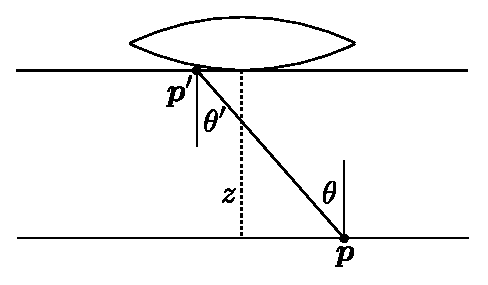
\includegraphics[width=0.5\linewidth]{chap06/Camerameasurementequation.eps}
    \caption{\refeq{6.5}辐射照度度量方程的几何设置。当辐射从
        尾部透镜元件切平面上的点$\bm p'$穿过到胶片平面上的点$\bm p$时可以被度量。
        $z$是从胶片平面到尾部元件切平面的轴向距离\refvar[LensRearZ]{RealisticCamera::LensRearZ}{()},
        而$\theta$是从$\bm p'$到$\bm p$的向量与光轴的夹角。}
    \label{fig:6.25}
\end{figure}

因为胶片平面平行\sidenote{译者注:原文误写为垂直,已修改。}于出射瞳平面,所以$\theta=\theta'$。
我们可进一步利用$\bm p$和$\bm p'$间的距离等于从胶片平面到出射瞳轴向距离
(这里我们表示为$z$)除以$\cos\theta$的事实。
将这些全部结合起来,我们有
\begin{align}\label{eq:6.5}
    E({\bm p})=\frac{1}{z^2}\int_{A_{\mathrm{e}}}{L_{\mathrm{i}}({\bm p},{\bm p}')|\cos^4\theta|\mathrm{d}A_{\mathrm{e}}}\, .
\end{align}

对于胶片范围相对于距离$z$较大的相机,项$\cos^4\theta$会
明显降低入射辐射照度——该因素也促成了暗角。
大多数现代数字相机都按照会增加传感器边缘像素值的预设校正因子来校正该效应。

胶片上一点的辐射照度对快门开启时间的积分
给出了\keyindex{注量}{fluence}{}
\sidenote{译者注:即\keyindex{辐射曝光量}{radiant exposure}{}。},
即单位面积上的辐射能量,单位$\text{J/m}^2$。
\begin{align}\label{eq:6.6}
    H({\bm p})=\frac{1}{z^2}\int_{t_0}^{t_1}\int_{A_{\mathrm{e}}}
    L_{\mathrm{i}}({\bm p},{\bm p}',t')|\cos^4\theta|\mathrm{d}A_{\mathrm{e}}\mathrm{d}t'\, .
\end{align}

度量一点的注量刻画了胶片平面接收的能量大小与相机快门开启的时长部分相关的效应。

摄影胶片(或者数字相机内的CCD\sidenote{译者注:即\keyindex{电荷耦合器件}{charge-coupled device}{}。}
或CMOS\sidenote{译者注:即\keyindex{互补式金属氧化物半导体}{complementary metal-oxide-semiconductor}{}。})
实际上是度量一小片面积上的辐射能量
\footnote{2015年代手机数字相机中像素的典型尺寸是每边1.5微米。}。
取\refeq{6.6}并在传感器像素面积$A_{\mathrm{p}}$上积分,我们有
\begin{align}\label{eq:6.7}
    J=\frac{1}{z^2}\int_{A_{\mathrm{p}}}\int_{t_0}^{t_1}\int_{A_{\mathrm{e}}}
    L_{\mathrm{i}}({\bm p},{\bm p}',t')|\cos^4\theta|\mathrm{d}A_{\mathrm{e}}\mathrm{d}t'\mathrm{d}A_{\mathrm{p}}\, ,
\end{align}
焦耳到达一个像素。

\refsec{蒙特卡洛估计器}中,我们将看到蒙特卡洛可以怎样运用于估计这些各种积分的值。
然后\refsub{采样相机1}中我们将定义\refvar{RealisticCamera::GenerateRay}{()}中的
代码片\refcode{Return weighting for RealisticCamera ray}{};
各种计算权重的方法允许我们计算这些量中的每一个。
\refsub{采样相机2}定义了相机模型的\keyindex{重要性函数}{importance function}{},
它表征了其对沿不同光线到达的入射光照的敏感性。